\chapter{Installation}
\label{chapter:Installation}
\index{Installation}

This section describes the process for installing OTB on your system.
OTB is a toolbox, and as such, once it is installed in your computer, it provides by default a set of useful libraries. You can use
these libraries to build your own applications based on it. What OTB does provide, besides the toolbox, is a
large set of test files and examples that will introduce you to OTB concepts
and will show you how to use OTB in your own projects.

Since the release 3.12, OTB embeds a specific framework to generate applications
in a more user-friendly way. OTB provides for each
application one shared library (also known as plugin). This plugin can be
auto-loaded into appropriate tools without recompiling, and is able to
fully describe its own parameters, behaviour and documentation.

The tools to use these plugins can be extended, but OTB is shipped with the
following:
\begin{itemize}
\item A command-line launcher,
\item A graphical launcher, with an auto-generated Qt interface,
  providing ergonomic parameters setting, display of documentation,
  and progress reporting,
\item A C and SWIG interface, which means that any application can be
  loaded, set up and executed into a high-level language such as \textbf{Python}
  for instance.
\end{itemize}

Based on a visualisation frammework which used FLTK libraries, Orfeo ToolBox team provides an integrated application which giving graphical access to a lot of OTB
functionalities: \textbf{Monteverdi}. Since mid-2013, we also provide a new grapical application based on Qt: \textbf{Monteverdi2}. This new application used the OTB-Applications tools as processing framework. 
   
There are two ways to install OTB on your system: installing from a binary distribution 
or compiling from sources. The choice depends on your system, and on what you intend to do.


\section{Installing binary packages}
\label{sec:install_binaries}

You can find all information about the installation of binary packages for OTB-Applications, Monteverdi and Monteverdi2 (if they are available on your platform) into the OTB-Cookbook.

The binary packages for OTB library are only available on:
\begin{itemize}
\item Ubuntu 12.04 and higher
\item OpenSuse 12.X and higher
\item MacOSX through MacPorts software  
\end{itemize}


\subsection{MacOS X}
\label{ssec:mac_binaries}

Orfeo Toolbox library is now available on \href{http://http://www.macports.org/}{MacPorts}.
The port name is called orfeotoolbox.
You can follow the \href{ http://guide.macports.org/}{MacPorts documentation} to install MacPorts first, then install the orfeotoolbox port.


\subsection{Ubuntu 12.04 and higher}
\label{ssec:ubuntu_binaries}
For Ubuntu 12.04 and higher, OTB and Monteverdi packages may be available as
Debian packages through APT repositories.

Since release 3.14.1, OTB packages are available in the
\href{https://launchpad.net/~ubuntugis/+archive/ubuntugis-unstable}{ubuntugis-unstable} repository.

You can add it by using these command-lines:
\begin{verbatim}
sudo aptitude install add-apt-repository
sudo apt-add-repository ppa:ubuntugis/ubuntugis-unstable
\end{verbatim}

Now run:
\begin{verbatim}
sudo aptitude update
\end{verbatim}
If you want only OTB libraries, please use:
\begin{verbatim}
sudo aptitude install libotb
\end{verbatim}

If you are using \emph{Synaptic}, you can add the repositories, update and install the packages through the
graphical interface.

For further informations about Ubuntu packages go to
\href{https://launchpad.net/~ubuntugis/+archive/ubuntugis-unstable}{ubuntugis-unstable}
launchpad page and click on \textbf{Read about installing}.
%% If you are using apt command-line tools, use these command-lines to add the otb repository to apt sources:
%% \begin{verbatim}
%% sudo aptitude install add-apt-repository
%% sudo add-apt-repository ppa:otb/orfeotoolbox-stable
%% \end{verbatim}


Moreover, \textbf{nightly} builds for all OTB projects are also available through APT repositories. However you should use it carefully. If you are using apt command-line tools, use these command-lines to add the otb repository to apt sources:

\begin{verbatim}
sudo aptitude install add-apt-repository
sudo add-apt-repository ppa:otb/orfeotoolbox-nightly
\end{verbatim}
Now run:
\begin{verbatim}
sudo aptitude update
\end{verbatim}
As with the previous cases, select which packages you will install.
\begin{verbatim}
sudo aptitude install libotb otb-bin otb-bin-qt python-otb monteverdi
\end{verbatim}

Be careful not to add the two repositories, since they may cause incompatibilities.

\textbf{apt-add-repository} will try to retrieve the GPG keys of the
repositories to certify the origin of the packages. If you are behind a http
proxy, this step won't work and apt-add-repository will stall and eventually
quit. You can temporarily ignore this error and proceed with the update
step. Following this, aptitude update will issue a warning about a signature
problem. This warning won't prevent you from installing the packages.

\subsection{OpenSuse 12.X and higher}
\label{ssec:opensuse_binaries}

For OpenSuse 12.X and higher, OTB and Monteverdi packages are available through
\emph{zypper}.

First, you need to add the appropriate repositories with these command-lines (please replace $11.4$ by your OpenSuse version):
\begin{verbatim}
sudo zypper ar
http://download.opensuse.org/repositories/games/openSUSE_11.4/ Games
sudo zypper ar
http://download.opensuse.org/repositories/Application:/Geo/openSUSE_11.4/ GEO
sudo zypper ar
http://download.opensuse.org/repositories/home:/tzotsos/openSUSE_11.4/ tzotsos
\end{verbatim}

Now run:
\begin{verbatim}
sudo zypper refresh
sudo zypper install OrfeoToolbox
sudo zypper install OrfeoToolbox-devel
\end{verbatim}

Alternatively you can use the One-Click Installer from the \href{http://software.opensuse.org/search?q=Orfeo&baseproject=openSUSE\%3A11.4&lang=en&include_home=true&exclude_debug=true}{openSUSE Download page} or add the above repositories and install through Yast Package Management.

In case you wish to test the latest version of the packages, you can run:
\begin{verbatim}
sudo zypper refresh
sudo zypper install OrfeoToolbox-beta
sudo zypper install OrfeoToolbox-beta-devel
\end{verbatim}

There is also support for the recently introduced 'rolling' openSUSE distribution named 'Tumbleweed'.
For Tumbleweed you need to add the following repositories with these command-lines:
\begin{verbatim}
sudo zypper ar
http://download.opensuse.org/repositories/games/openSUSE_Tumbleweed/ Games
sudo zypper ar
http://download.opensuse.org/repositories/Application:/Geo/openSUSE_Tumbleweed/ GEO
sudo zypper ar
http://download.opensuse.org/repositories/home:/tzotsos/openSUSE_Tumbleweed/ tzotsos
\end{verbatim}
and then add the OTB packages as shown above.


\section{Building from sources}
\label{sec:source}
OTB has been developed and tested across different combinations of
operating systems, compilers, and hardware platforms including
MS-Windows, Linux on Intel-compatible hardware and Mac
OSX.  It is known to work with the following compilers:
\begin{itemize}
\item Visual Studio C++ 9.0 .NET 2008, Visual Studio Express 2008 and 2010 on MS-Windows
\item GCC (4.1, 4.2, 4.3, 4.4, 4.5, 4.6, 4.7) on Unix/Linux systems
\item GCC on MacOSX (10.6 and higher) systems
\end{itemize}

Given the advanced usage of C++ features in the toolbox, some
compilers may have difficulties processing the code. If you are
currently using an outdated compiler this may be an excellent excuse
for upgrading this old piece of software!

Please note that even if this section only describes how to compile OTB from sources,
Monteverdi can be compiled in a similar way.

\subsection{Getting the OTB source code}

There are three ways of getting the OTB source code:
\begin{itemize}
\item Download the latest current release from the \href{http://sourceforge.net/projects/orfeo-toolbox/}{OTB download page},
\item Clone the current release with \href{http://mercurial.selenic.com}{Mercurial} from the \href{http://hg.orfeo-toolbox.org/OTB}{OTB mercurial server},
\item Clone the latest revision with \href{http://mercurial.selenic.com}{Mercurial} from the \href{http://hg.orfeo-toolbox.org/OTB}{OTB mercurial server}.
\end{itemize}

These last two options need a proper \href{http://mercurial.selenic.com}{Mercurial} installation. To get source code from Mercurial, do:
\begin{verbatim}
hg clone http://hg.orfeo-toolbox.org/OTB
\end{verbatim}

Using Mercurial, you can easily navigate through the different version. For instance, this brings you to the 3.16.0 source code version:
\begin{verbatim}
hg update -r 3.16.0
\end{verbatim}

And this brings you to the latest development version:
\begin{verbatim}
hg update
\end{verbatim}


\subsection{External Libraries}

The OTB depends on several libraries:
\begin{itemize}
\item ITK: The medical image processing library is embedded in the OTB, it is considered as an internal library.
\item GDAL: The support of remote sensing imagery formats is ensured
  through the use of the GDAL library. Please see
  \url{http://www.remotesensing.org/gdal/} for informations on how to install.
\item OSSIM: Image geometry library, it handles for example the sensor geometric models.
  Please see \url{http://www.ossim.org} for informations on how to install.
download and install this library on your system. OTB requires at least the version 1.6.
\item Fltk: this library is used for the visualization
  functionnalities. See \url{http://www.fltk.org/} for details about
  dowloading and installing Fltk. OTB has been tested with version 1.1.9,
  1.1.10 and 1.3. You also have the choice to use OTB's internal
  version (which is 1.1.9) if you don't have FLTK already installed.
\item gettext (optional): Since version 3.2, OTB includes experimental support
  for internationalization. Gettext is required to activate this
  functionnality.
\end{itemize}

See section \ref{sec:FAQInstall} for quick installation guidelines for GDAL or Fltk if you don't have access
to standard packages.

\subsection{Configuring OTB}
\label{sec:ConfiguringOTB}

\index{Configuration}

The challenge of supporting OTB across platforms has been solved through the
use of CMake, a cross-platform, open-source build system. CMake is used to
control the software compilation process using simple platform and compiler
independent configuration files.  CMake generates native makefiles and
workspaces that can be used in the compiler environment of your choice. CMake
is quite sophisticated---it supports complex environments requiring system
configuration, compiler feature testing, and code generation.

CMake generates Makefiles under UNIX systems and generates Visual
Studio workspaces under Windows (and appropriate build files for other
compilers like Borland). The information used by CMake is provided by
\code{CMakeLists.txt} files that are present in every directory of the OTB
source tree. These files contain information that the user
provides to CMake at configuration time. Typical information includes paths
to utilities in the system and the selection of software options specified by
the user.

\subsubsection{Preparing CMake}
\label{sec:CMakeforOTB}

\index{CMake}
\index{CMake!downloading}

CMake can be downloaded at no cost from
\begin{center}
  \url{http://www.cmake.org}
\end{center}

OTB requires at least CMake version 2.8. You can download binary
versions for most of the popular platforms including Windows, Solaris,
IRIX, HP, Mac and Linux. Alternatively you can download the source
code and build CMake on your system. Follow the instructions in the
CMake Web page for downloading and installing the software.

For Unix/Linux systems, an additional help can be found, to compile Cmake from source, in the \ref{sec:FAQInstall}
section, subsection Unix/Linux Platforms.

\index{CMake!OTB tree}
Running CMake initially requires that you provide two pieces of
information:
\begin{itemize}
\item Where the source code directory is located (ex.: OTB\_SOURCE\_DIR),
\item Where the object code is to be produced: (ex.: OTB\_BINARY\_DIR).
\end{itemize}
These are referred to as the \emph{source directory} and the \emph{binary directory}.
We recommend setting the binary directory to be different than the source directory (an
\emph{out-of-source} build), but OTB will still build if they are set
to a directory inside the source directory (an \emph{in-source} build).

\subsubsection{Compiling OTB}
CMake runs in an interactive mode in that you iteratively select
options and configure according to these options. The iteration
proceeds until no more options remain to be selected. At this point, a
generation step produces the appropriate build files for your
configuration.

This interactive configuration process can be better understood if you
imagine that you are walking through a decision tree.  Every option that you
select introduces the possibility that new, dependent options may become
relevant. These new options are presented by CMake at the top of the options
list in its interface.  Only when no new options appear after a configuration
iteration can you be sure that the necessary decisions have all been made. At
this point build files are generated for the current configuration.

As the following figures display it, CMake has a different interface according to your systems.
\label{sec:ConfiguringOTBwithVTK}
\index{Configuration!with VTK}

\begin{figure}[ht]
\centering
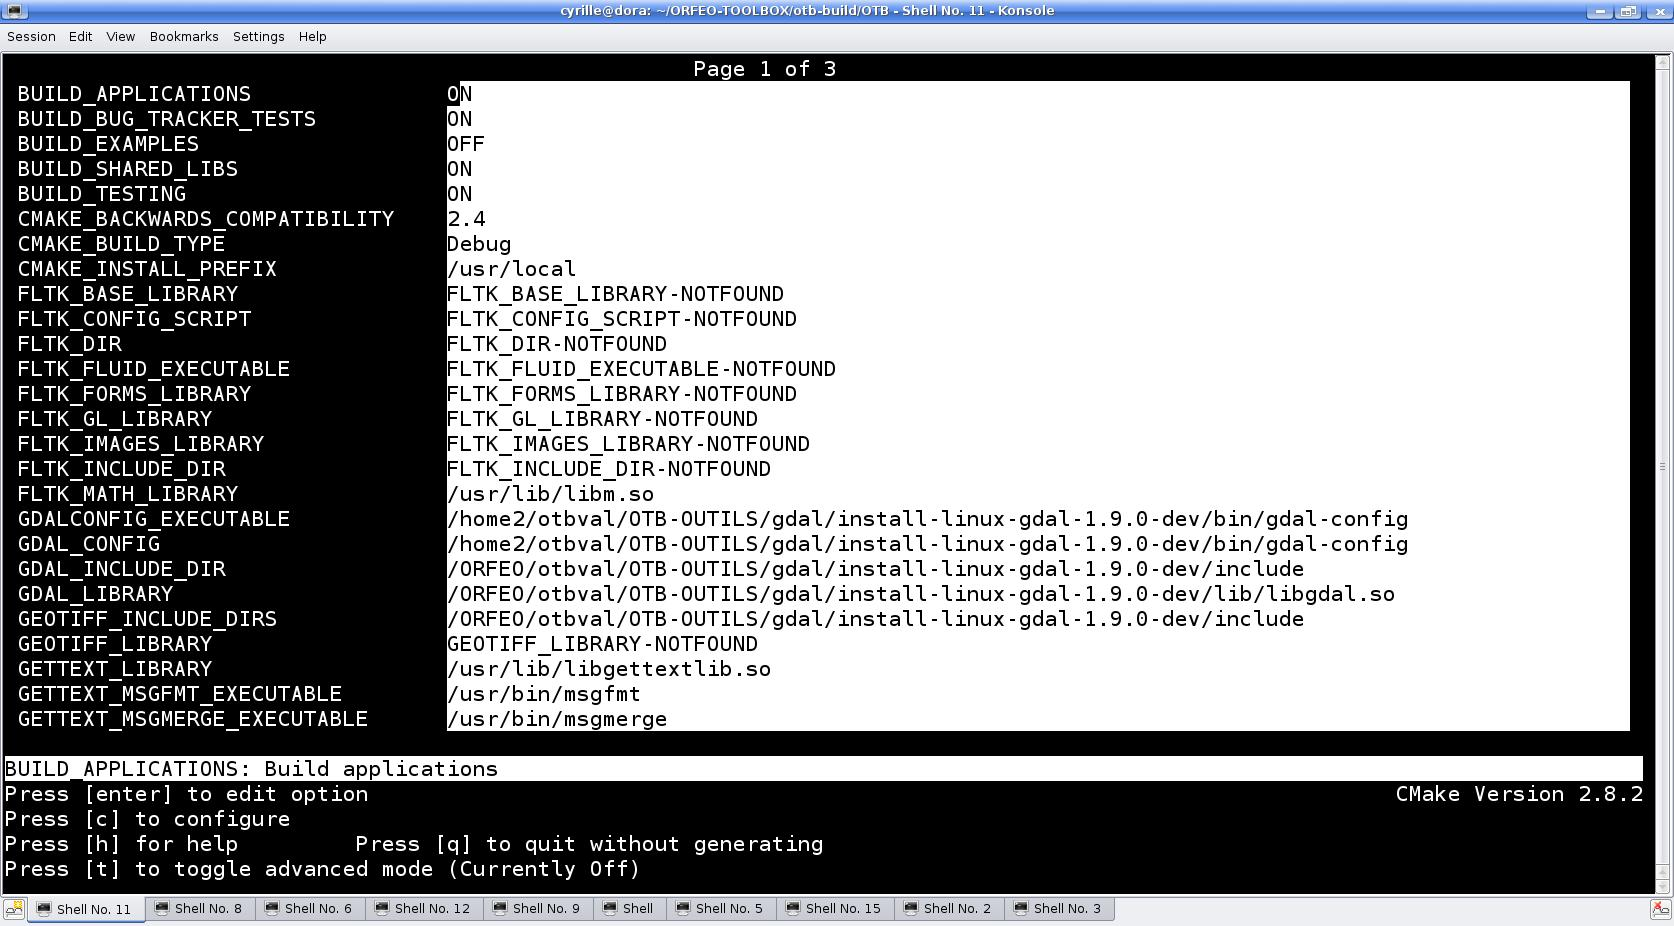
\includegraphics[width=0.8\textwidth]{ccmakeScreenShot.eps}
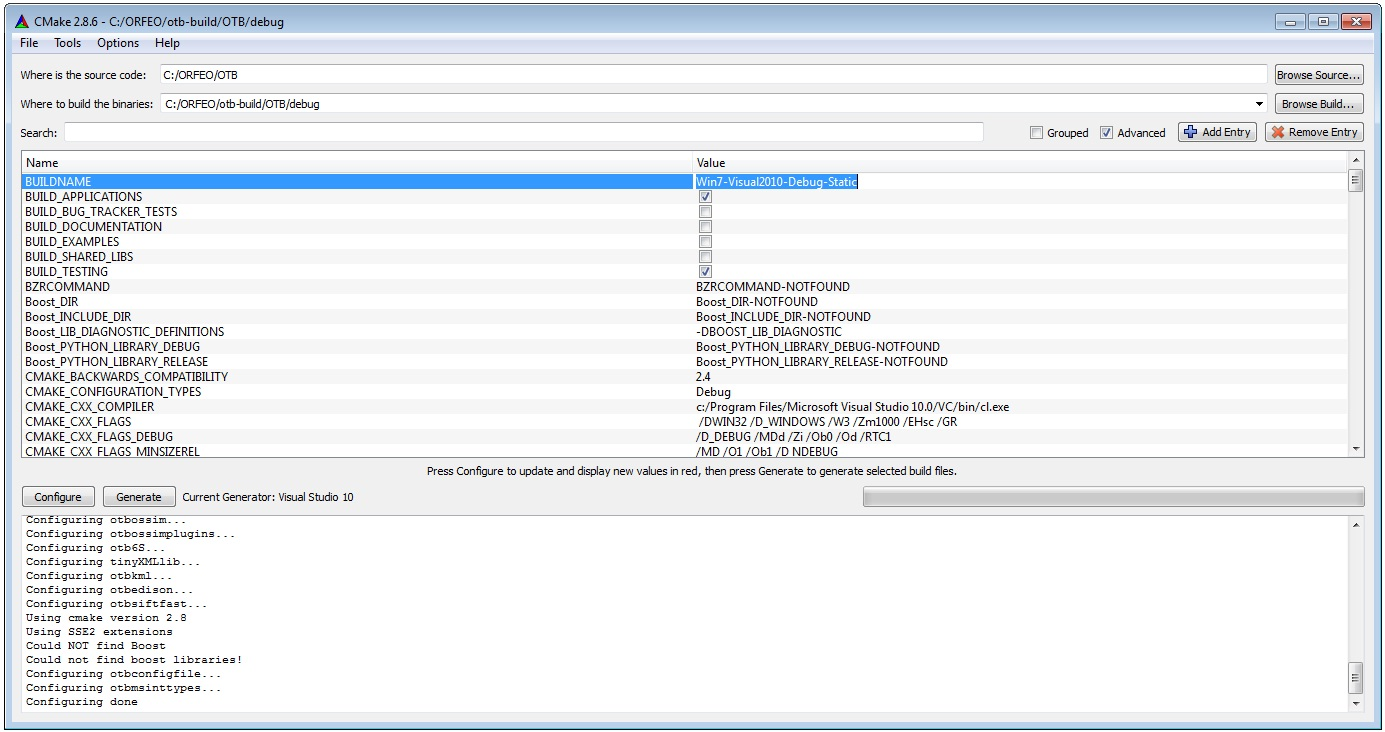
\includegraphics[width=0.8\textwidth]{CMakeSetupScreenShot.eps}
\itkcaption[Cmake user interface]{CMake interface. Top) \texttt{ccmake}, the UNIX
version based on \texttt{curses}. Bottom) \texttt{CMakeSetup}, the MS-Windows
version based on MFC.}
\label{fig:CMakeGUI}
\end{figure}


\textbf{\underline{On Windows:}}
\index{Downloading libraries from OSGeo4W}
The OTB needs some external libraries to work, as described in the table \ref{tab:installation2} of section \ref{sec:FAQInstall}. On Windows, we recommended to use the OSGeo4W tool to get those libraries. However, as several of these libraries are optional or internal to OTB, the minimum requirement for compiling OTB is to install Gdal.
\begin{enumerate}
\item Download and start the OSGeo4w setup in advanced mode
\item Select the gdal package located in Libs folder
\item Optionally select the other libraries you want to use as external
\item Proceed with the installation.
\end{enumerate}

\index{Configuring CMake on Windows}
On windows, you will first create a directory to hold the binaries to be built.
Your directory structure may look as follows:
\begin{verbatim}
* OTB
|- OTB_SOURCE_DIR
|- OTB_BINARY_DIR
\end{verbatim}
where \texttt{OTB\_SOURCE\_DIR} contains is the base directory of the OTB source code, and
\texttt{OTB\_BINARY\_DIR} is empty for now.

Launch the CMake executable. On the top of the GUI (Figure \ref{fig:CMakeGUI}), select the source and binary directories, then press \emph{Configure}.
Variables appear at the center of the CMake GUI. You must set some of these variables to tell CMake about your system. The first thing to do is to enable the \emph{Advanced} checkbox and change the value of the \texttt{OSGEO4W\_ROOT} variable to the directory where you installed OSGeo4W. Then press \emph{Configure} again.

The \emph{Generate} button will be accessible only when all required CMake variables are correctly set. At this time, push \emph{Generate}, wait for the end of the generation process then close the CMake window.

\index{Compiling OTB on Windows}
Now, you can go in your \emph{binary directory} (here \texttt{OTB\_BINARY\_DIR}). CMake has generated Makefiles or
Visual Studio project files. You can open the solution and build the \texttt{ALL\_BUILD} project.
If you plan to run executables from within the Visual Studio environment, you should open the Visual Studio
solution file from the OSGeo4W shell. To do this, simply drag-and-drop the ".sln" file to an OSGeo4W shell
and press Enter.

Windows platforms didn't support to build with shared libraries. If you experience any problem
with that, you can set \texttt{BUILD\_SHARED\_LIBS} to \texttt{OFF} but the
built size might reach 1~GB.

That should be all! Otherwise, subscribe to
otb-users@googlegroups.com and you will get some help.

\textbf{\underline{On Linux/Unix:}}
\index{Configuring CMake on Unix}
On Unix, the binary directory is created by the user and CMake is invoked with the
path to the source directory. For example:
\small
\begin{verbatim}
mkdir OTB_BINARY_DIR
cd OTB_BINARY_DIR
ccmake ../OTB_SOURCE_DIR
\end{verbatim}
\normalsize

Once the interface open, you can push \emph{c} (for Configure), or/and \emph{t} for Toggle (to have access to the advanced variables). If you have follow the section \ref{sec:FAQInstall} every needed libraries are in the
\emph{/usr} and will be found automatically by CMake. Set the following recommended CMake variables:
\begin{itemize}
\item OTB\_USE\_EXTERNAL\_BOOST:BOOL=ON
\item OTB\_USE\_CURL:BOOL=ON
\item OTB\_USE\_EXTERNAL\_EXPAT:BOOL=ON
\item OTB\_USE\_LIBLAS:BOOL=ON
\item OTB\_USE\_EXTERNAL\_LIBLAS:BOOL=ON
\item OTB\_USE\_GETTEXT:BOOL=OFF
\item OTB\_USE\_JPEG2000:BOOL=ON
\end{itemize}

Push \emph{c} to update CMake untill the option \emph{Generate} is accessible in the GUI,
then push \emph{g} fot \emph{Generate}. The CMake interface will close itself.
Then, go into your build directory (here OTB\_BINARY\_DIR) and do \emph{make} to launch the compilation.

If you want to put OTB in a standard location, you can proceed with:

\begin{verbatim}
make install
\end{verbatim}

\textbf{\underline{Compilation awarness}}
The build process will typically take anywhere from 15 to 30 minutes depending
on the performance of your system. If you decide to enable testing as part of
the normal build process, about 2500 small tests programs will be compiled. This
will verify that the basic components of OTB have been correctly built on your
system.

Set the CMake variables \code{BUILD\_TESTING} and \code{BUILD\_EXAMPLES} to ON will activate
the compilation of the examples and the tests and slow down the build process.
The examples distributed with the toolbox are a helpful resource for learning how to use OTB
components but are not essential for the use of the toolbox itself. The testing
section includes a large number of small programs that exercise the
capabilities of OTB classes. Due to the large number of tests, enabling the
testing option will considerably increase the build time.  It is not
desirable to enable this option for a first build of the toolbox.

Set the CMake variable \code{BUILD\_APPLICATION} to ON will activate the compilation of the applications and their launchers needed to use it. A complete list of these applications, described in the OTB Cookbook, can be found on \href{http://orfeo-toolbox.org/Applications/index.html}{OTB Website}.



\section{Getting Started With OTB }
\label{sec:GettingStartedWithOTB}

The simplest way to create a new project with OTB is to create a new directory
somewhere in your disk and create two files in it. The first one is a
\code{CMakeLists.txt} file that will be used by CMake to generate a Makefile
(if you are using UNIX) or a Visual Studio workspace (if you are using
MS-Windows).  The second file is an actual C++ program that will exercise
some of the large number of classes available in OTB. The details of these files
are described in the following section.

Once both files are in your directory you can run CMake in order to configure
your project. Under UNIX, you can cd to your newly created directory
and type ``\code{ccmake .}''. Note the ``.'' in the command line for indicating
that the \code{CMakeLists.txt} file is in the current directory. The
curses interface will require you to provide the directory where OTB
was built. This is the same path that you indicated for the
\code{OTB\_BINARY\_DIR} variable at the time of configuring OTB. Under
Windows you can run CMakeSetup and provide your newly created
directory as being both the source directory and the binary directory for
your new project (i.e., an in-source build). Then CMake will require you to
provide the path to the binary directory where OTB was built. The OTB binary
directory will contain a file named \code{OTBConfig.cmake} generated during the
configuration process at the time OTB was built.  From this file, CMake will
recover all the information required to configure your new OTB project.


\subsection{Hello World !}
\label{sec:HelloWorldOTB}

\index{Hello World}

Here is the content of the two files to write in your new project. These two
files can be found in the \code{OTB/Examples/Installation} directory. The
\code{CMakeLists.txt} file contains the following lines:

\small
\begin{verbatim}
PROJECT(HelloWorld)

FIND_PACKAGE(OTB REQUIRED)
INCLUDE(${OTB_USE_FILE})

ADD_EXECUTABLE(HelloWorld HelloWorld.cxx )
TARGET_LINK_LIBRARIES(HelloWorld OTBIO)
\end{verbatim}

\normalsize

The first line defines the name of your project as it appears in Visual
Studio (it will have no effect under UNIX). The second line loads a CMake
file with a predefined strategy for finding OTB \footnote{Similar files are
provided in CMake for other commonly used libraries, all of them named
\code{Find*.cmake}}. If the strategy for finding OTB fails, CMake will prompt
you for the directory where OTB is installed in your system. In that case you
will write this information in the \code{OTB\_DIR} variable. The line \code{
INCLUDE(\$\{USE\_OTB\_FILE\})} loads the \code{UseOTB.cmake} file to set
all the configuration information from OTB.

%The next block of lines is needed in order for CMake to know whether you
%are using the OTB's internal version of ITK or an external one. In the
%second case, CMake will try to find ITK in your system. As for OTB, if
%it fails in finding ITK, it will ask you to manually set the ITK location.

The line \code{ADD\_EXECUTABLE}
defines as its first argument the name of the executable that will be produced
as result of this project. The remaining arguments of \code{ADD\_EXECUTABLE}
are the names of the source files to be compiled and linked.  Finally, the
\code{TARGET\_LINK\_LIBRARIES} line specifies which OTB libraries will be
linked against this project.


\input HelloWorld.tex

At this point you have successfully installed and compiled OTB, and created
your first simple program. If you have difficulties, please join the
otb-users mailing list (Section~\ref{sec:JoinMailList} on page
\pageref{sec:JoinMailList}) and post questions there.
